% Main empirical-section paragraph.
Table~\ref{tab:ritz-certification-main} reports finite-rank approximation errors and Ritz bounds for the principal stress probe in each application at $\lambda_0=1$. The exact error column compares the rank-$R$ Ritz approximation with the full-coordinate stress statistic. The Ritz bound is a deterministic certification bound conditional on the estimated covariance operators. It is intentionally conservative: it combines omitted probe mass with a residual term for the Ritz subspace and is capped at one, so entries marked as vacuous should not be read as evidence that the approximation error is large.

The rows are probe-specific. A low-rank approximation can be accurate for one stress probe while remaining uncertified or inaccurate for another. This is especially important in the hurricane appendix, where the 72-dimensional full-surface rows use a fiscal/post block probe, whereas the restricted 28-dimensional fiscal/post rows use the restricted surface's whole-surface soft probe.

The macro benchmark is a full-space temporal-resolvent benchmark, $K_\eta(t)=\sum_j W_{\eta,tj}\chi_j\chi_j'$, rebuilt from the original 125-dimensional pre-PCA influence contributions. It is not a full-dimensional latent state-space fit. The stress curves in Figure~\ref{fig:macro-ritz-interval-spectrum} use the ridge-adjusted reference scale. Dashed curves are unnormalized rank-five Ritz approximations to the full $Q_\rho$ stress, not legacy trace-normalized rank-five stress statistics.

The temporal-resolvent smoothing parameter is selected by blocked predictive Gaussian quasi-likelihood on the saved eta grid. The metadata reports whether the selected value is an interior or boundary solution and lists the best neighboring candidates. Severe-direction counts, Ritz errors, subspace capture, and plotted stress variation are reported only after selection and do not enter the eta criterion.

Severe-direction diagnostics ask a different question from stress approximation. They count generalized eigen-directions whose ridge-adjusted amplification exceeds a threshold and then report how much of those eigenspaces is captured by the leading empirical covariance subspace. Low capture means that high-amplification directions are geometrically different from the leading covariance directions, even when exact low-rank stress errors appear moderate.

% Appendix inclusions.
\begin{table}[!htbp]
\centering
\caption{Finite-rank approximation errors and Ritz bounds}
\label{tab:ritz-certification-main}
\resizebox{\linewidth}{!}{%
\begin{tabular}{@{}llrrrrrr@{}}
\toprule
Application & Probe & $p$ & $R$ & Retained mass & p95 $e_R$ & $\max e_R$ & $\max B_R$ \\
\midrule
LaLonde ATE & overall ATE direction & 11 & 5 & 0.999 & 0.007 & 0.011 & 0.805 \\
Hurricane full fiscal/post probe & fiscal/post block probe & 72 & 5 & 0.661 & 0.178 & 0.214 & 1.000 (vacuous) \\
Hurricane full fiscal/post probe & fiscal/post block probe & 72 & 15 & 0.869 & 0.056 & 0.065 & 1.000 (vacuous) \\
\bottomrule
\end{tabular}
}
\begin{minipage}{0.96\linewidth}
\footnotesize Notes: $e_R$ is the exact full-coordinate stress approximation error at $\lambda_0=1$ and $B_R$ is the capped deterministic Ritz bound. The macro row uses the full-space temporal-resolvent benchmark built from 125-dimensional pre-PCA influence contributions; it is not a full-dimensional latent state-space estimate. Bounds are conditional on the estimated regularized covariance operators.
\end{minipage}
\end{table}


\begin{figure}[!htbp]
\centering
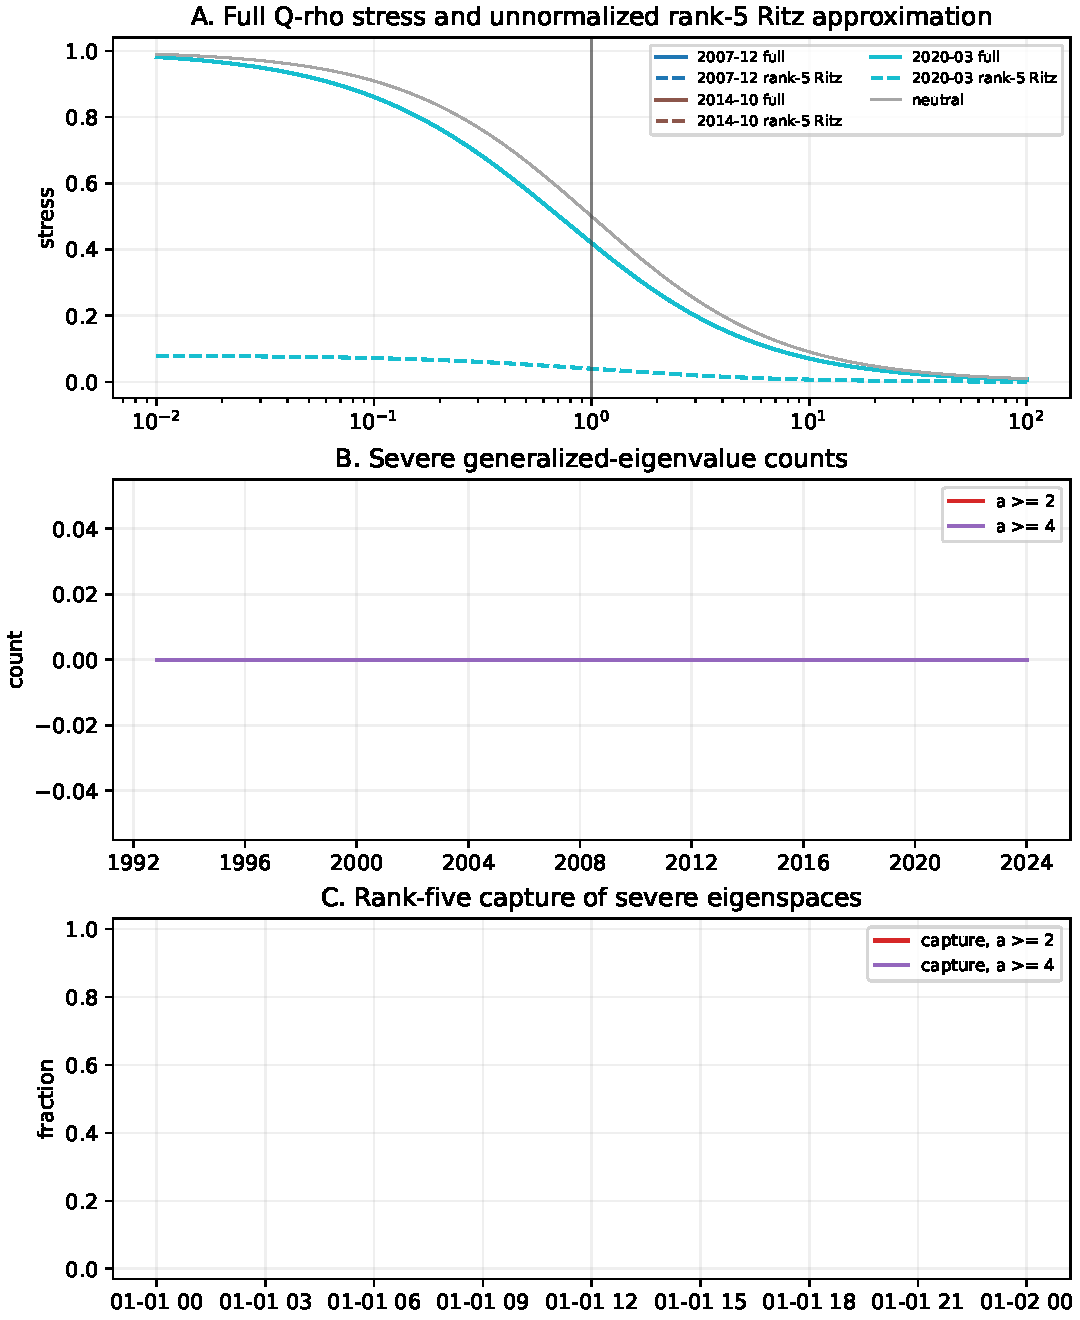
\includegraphics[width=0.96\linewidth]{results/ritz_certification/figures/macro_ritz_interval_spectrum.pdf}
\caption{Macro Ritz stress and interval-spectrum diagnostics. Notes: the full calculation is a 125-dimensional temporal-resolvent benchmark, not a full-dimensional version of the nonlinear rank-five latent state-space model. Eta is selected by blocked predictive Gaussian quasi-likelihood on held-out full influence vectors; the metadata reports whether the selected value is a boundary solution. The rank-five curve compresses the same ridge-relative operator. Amplification thresholds are relative to $\widehat C+\rho I$ and are therefore ridge-adjusted. The interval-spectrum backend is \texttt{scipy.linalg.eigh(..., subset\_by\_value=...)}, with the maximum generalized-eigenpair residual reported in metadata.}
\label{fig:macro-ritz-interval-spectrum}
\end{figure}

\begin{table}[!htbp]
\centering
\caption{Hurricane Ritz certification and severe-direction geometry}
\label{tab:hurricane-ritz-certification}
\scriptsize
\textbf{Panel A. Accuracy}\\[0.3em]
\resizebox{\linewidth}{!}{%
\begin{tabular}{@{}llrrrrrr@{}}
\toprule
Surface and rank & Probe & Trace share & Retained mass & p95 $e_R$ & $\max e_R$ & Share $e_R>.05$ & p95 Ritz subspace residual term \\
\midrule
72-coordinate full event-study surface, R=5 & fiscal/post block probe & 0.603 & 0.661 & 0.178 & 0.214 & 0.718 & 2.716 \\
72-coordinate full event-study surface, R=10 & fiscal/post block probe & 0.723 & 0.759 & 0.135 & 0.144 & 0.574 & 4.298 \\
72-coordinate full event-study surface, R=15 & fiscal/post block probe & 0.807 & 0.869 & 0.056 & 0.065 & 0.133 & 3.971 \\
28-coordinate fiscal/post event-study surface, R=5 & whole-surface soft probe & 0.731 & 0.190 & 0.489 & 0.502 & 1.000 & 1.953 \\
28-coordinate fiscal/post event-study surface, R=10 & whole-surface soft probe & 0.902 & 0.379 & 0.366 & 0.373 & 1.000 & 3.490 \\
28-coordinate fiscal/post event-study surface, R=15 & whole-surface soft probe & 0.964 & 0.567 & 0.259 & 0.294 & 0.877 & 2.564 \\
\bottomrule
\end{tabular}
}
\\[0.8em]
\textbf{Panel B. Severe Geometry}\\[0.3em]
\resizebox{\linewidth}{!}{%
\begin{tabular}{@{}lrrrrrr@{}}
\toprule
Surface and threshold & Median $d$ & Max $d$ & Share $d>0$ & Median $\kappa$ & p90 $\kappa$ & Max generalized-eigenpair residual \\
\midrule
72-coordinate full event-study surface, $a_\star=2$ & 10.000 & 23 & 0.959 & 0.013 & 0.144 & 3.2e-13 \\
72-coordinate full event-study surface, $a_\star=4$ & 3.000 & 12 & 0.836 & 0.006 & 0.301 & 3.2e-13 \\
28-coordinate fiscal/post event-study surface, $a_\star=2$ & 2.000 & 15 & 0.621 & 0.108 & 0.337 & 1.4e-13 \\
28-coordinate fiscal/post event-study surface, $a_\star=4$ & 0.000 & 7 & 0.441 & 0.226 & 0.685 & 1.4e-13 \\
\bottomrule
\end{tabular}
}
\begin{minipage}{0.96\linewidth}
\footnotesize Notes: The restricted surface is the true fiscal/post intersection derived from checked-in surface metadata. Panel A's residual term is $r_R(s)/\lambda$ with $\lambda=1$, where $r_R(s)$ is the Ritz subspace residual. Panel B defines $\kappa_5(s;a_\star)=\|V_5'U_\star(s)\|_F^2/d_\star(s;a_\star)$ when $d_\star>0$. Interval eigenpairs are extracted with \texttt{scipy.linalg.eigh(..., subset\_by\_value=...)} and verified against full dense eigenvalue counts; the reported residual is the numerical generalized-eigenpair residual.
\end{minipage}
\end{table}


\begin{figure}[!htbp]
\centering
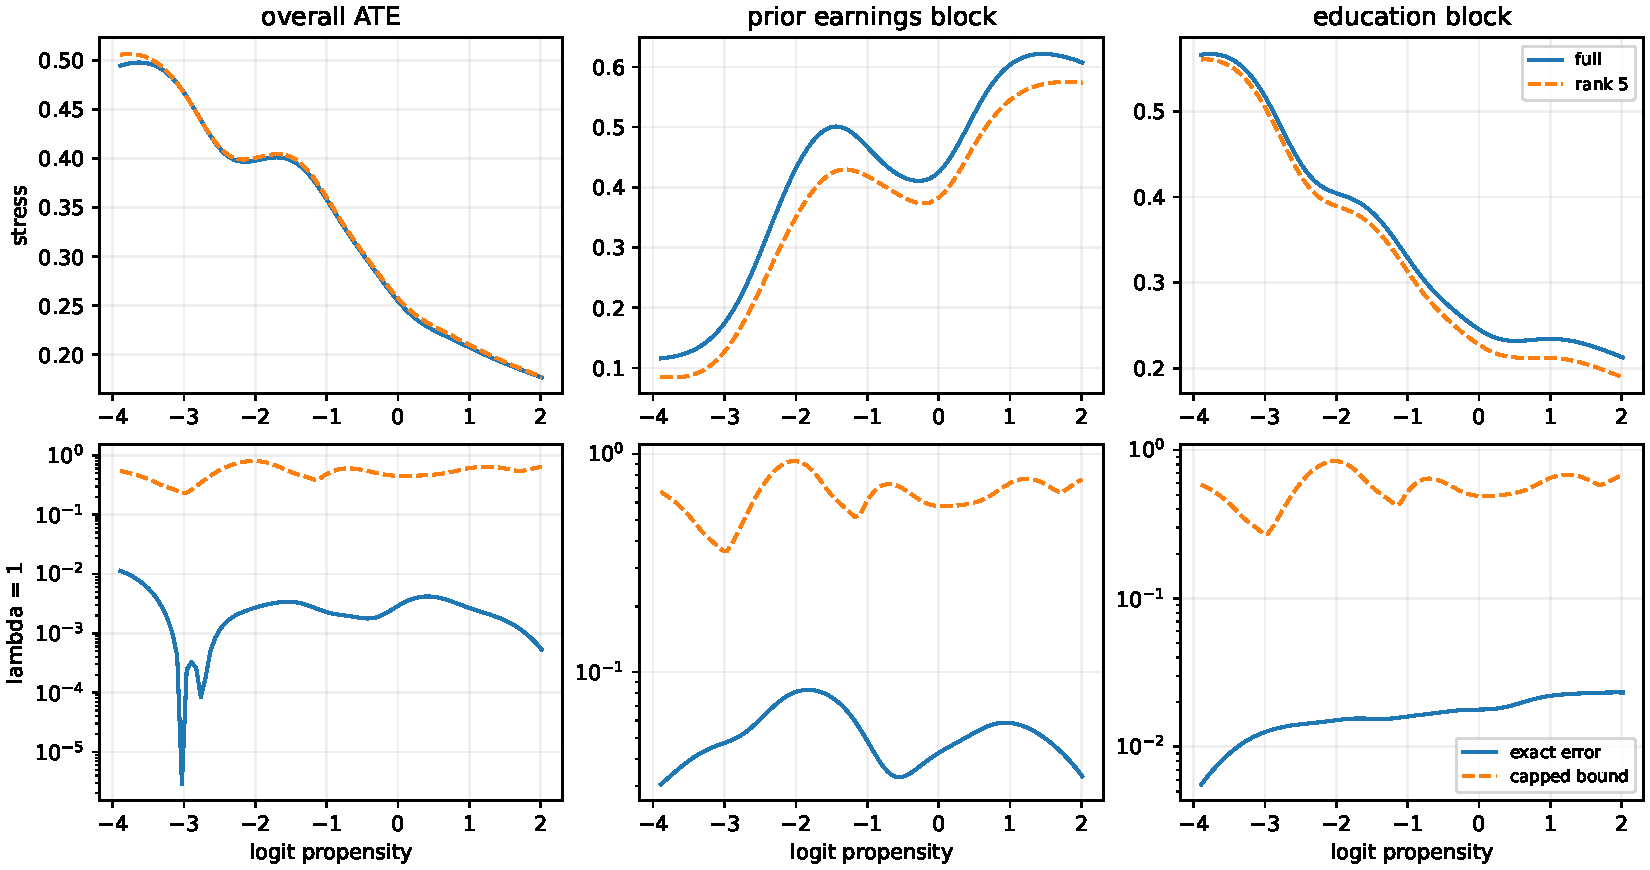
\includegraphics[width=0.96\linewidth]{results/ritz_certification/figures/lalonde_ritz_validation.pdf}
\caption{LaLonde Ritz-bound validation. The lower row uses a log scale so the exact rank-five errors remain visible against the deterministic Ritz certificates.}
\label{fig:lalonde-ritz-validation}
\end{figure}
